As can be seen in fig. \ref{fig:4mic1srcInd}, even in ideal conditions, the localization results from SRP-PHAT contain many peaks of varying heights. This is due to summing the cross-correlation responses of a non-linear array (Eq. \ref{eq:srpSumInd}). If the array was linear, the localization circles from each pair would all overlap completely. In case of a tetrahedral array, the localization circles from the possible microphone pairs are not co-planar. This is because all the edges of a tetrahedron point in the different directions. The obvious problem here is in multi-source detection. If multiple sources are playing at different levels, how do we determine if a detected peak is a real source or a pseudo-source from another higher level source? The methods to do so form the basis of deconvolution methods for SRP-PHAT.

\subsection{Deconvolution of the array response}

Deconvolution methods has been applied in several different area over the last years. The CLEAN algorithm proposed by Jan Högbom in 1974 \cite{1974A&AS...15..417H} performs the deconvolution of images in radio astronomy. Högbom observed the sky images being polluted by what he described as the "dirty beam". This "dirty beam" is the distortion introduced in the system output when the input is subject to a point source. The CLEAN algorithm removes the side lobes of the beamformer when the PSF is known in advance throught simulation or measurement. CLEAN-SC is an extension of the CLEAN algorithm which uses the coherence between the sidelobes and the main beam to remove the PSF and retrieve the level of the sources. Other methods such as DAMAS or DAMAS-SC rely on the Cross Spectrum Matrix (CSM) to solve a set of linear equations. Computing the CSM is usually done for a single frequency whereas our algorithm should be able to perform on a wide band. Some method also rely on frequency domain beamforming where efficient deconvolution can be performed (shift-invariant PSF). In our case the array response change for every scanned position and the beamforming is performed in the time domain therefore those techniques are not discarded. Other methods to perform the deconvolution in the time domain are discussed in the following part such as product SRP-PHAT and minimum power SRP-PHAT. Minimum power SRP-PHAT application proved successfull to clean the map while maintaining accurate level difference between multiple sources. Those methods have also proven to be resilient to adverse conditions (high noise, inaccurate microphone positions, wind)

\newpage
\subsubsection{Product-SRP-PHAT}
A simple deconvolution approach could be to penalize sources which are only detected by a subset of the microphone pair combinations. This could be done by taking a product and not a sum in Eq. \ref{eq:srpSumInd}.
\begin{equation}
    S_{SRP}(\theta,\phi)=\prod\limits_{i=1}^{M-1}{R_{x_0,x_i}[f_{0,i}(\theta,\phi)]}
     \label{eq:srpProdInd}
\end{equation}
This way, if a peak is caused by a single localization circle, the cross-correlation values from other microphone pairs would be close to zero, and thus would scale the false peak down. The localization results from this are given in fig. \ref{fig:4mic1srcNoisyProd}.
\begin{figure}[H]
    \centering
    \begin{subfigure}[b]{0.96\textwidth}
    \centering
    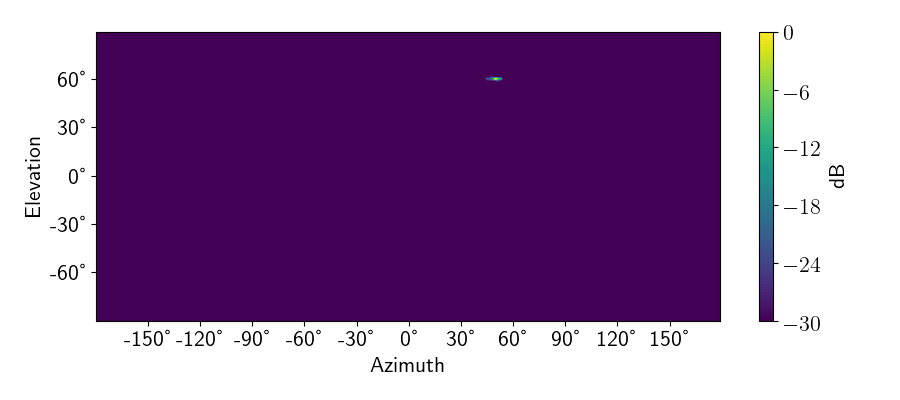
\includegraphics[width=0.8\textwidth]{Figures/Ind4mic1srcProd20.png}
\end{subfigure}
\vskip \baselineskip
\begin{subfigure}[b]{0.96\textwidth}
    \centering
    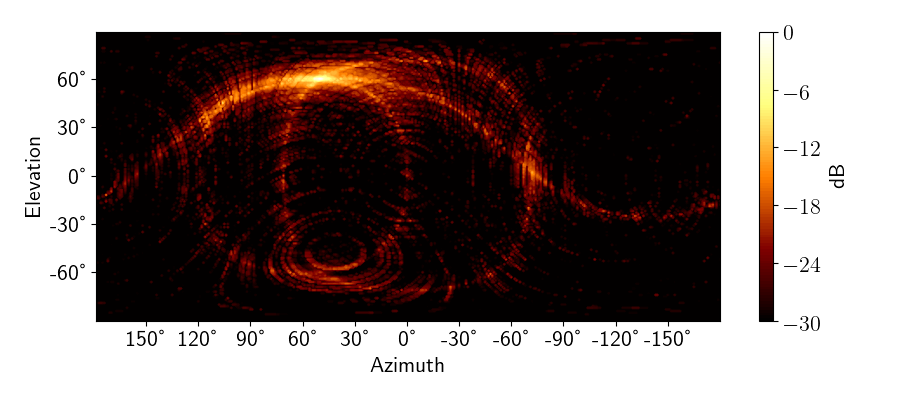
\includegraphics[width=0.8\textwidth]{Figures/Ind4mic1srcProd0.png}
\end{subfigure}
\vskip \baselineskip
\begin{subfigure}[b]{0.96\textwidth}
    \centering
    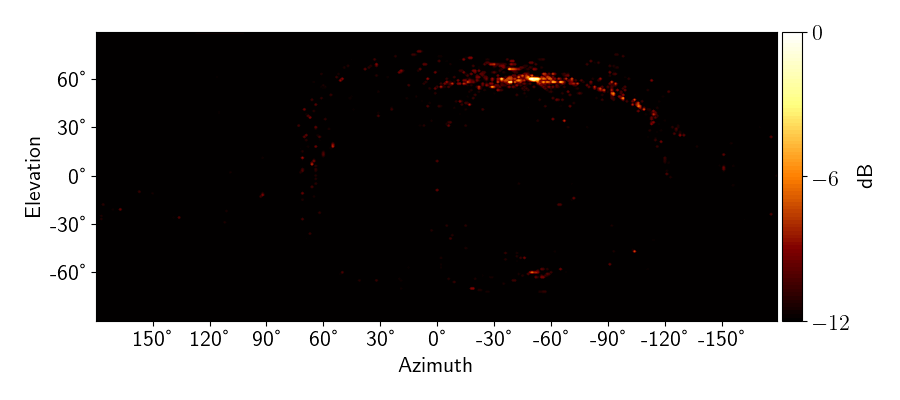
\includegraphics[width=0.8\textwidth]{Figures/Ind4mic1srcProdNeg10.png}
\end{subfigure}
\caption{Figures depict from top-to-bottom product-SRP-PHAT localization results  with SNR = 20dB, SNR = 0dB, SNR = -10dB}
\label{fig:4mic1srcNoisyProd}
\end{figure}
\newpage
The drawback of using product-SRP-PHAT is that the sound level difference between the different sound sources is lost. In normal SRP-PHAT, the array magnitude response at a particular azimuth and elevation is averaged over all microphone pair combinations. Then the level difference between 2 sources is maintained. In product-SRP-PHAT this would not be the case. However if it is assumed that a particular source will have similar magnitude response for all microphone pairs (which is not a strong assumption in far-field), then taking source power $P_{SRP}={S_{SRP}}^{1/M}$, the level difference can be maintained.  Fig. \ref{fig:4mic2srcNoisyCompare} depicts the results of product-SRP-PHAT after level correction.
\begin{figure}[H]
    \centering
    \begin{subfigure}[b]{0.96\textwidth}
    \centering
    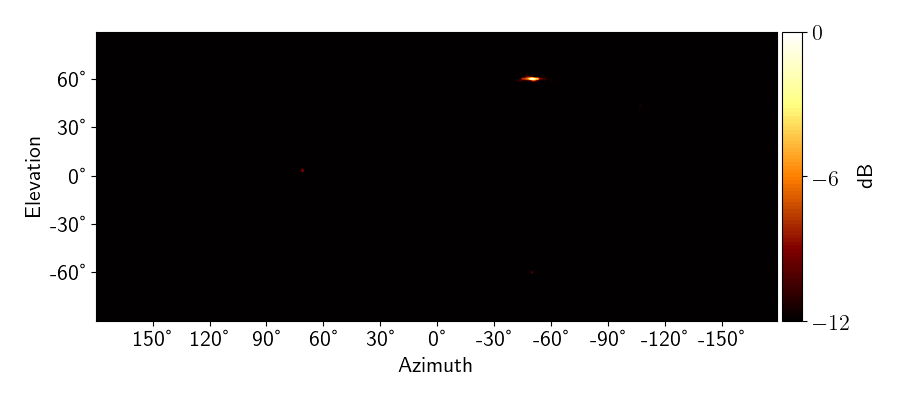
\includegraphics[width=0.8\textwidth]{Figures/Ind4mic1srcProd20Corr.png}
\end{subfigure}
\vskip \baselineskip
\begin{subfigure}[b]{0.96\textwidth}
    \centering
    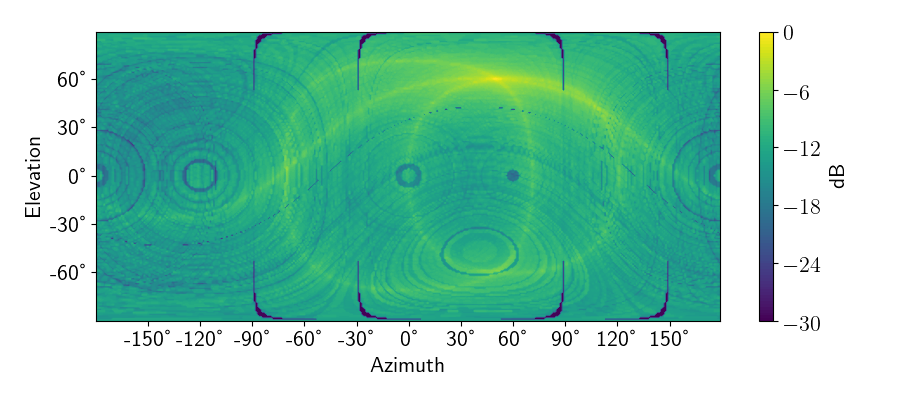
\includegraphics[width=0.8\textwidth]{Figures/Ind4mic1srcProd0Corr.png}
\end{subfigure}
\vskip \baselineskip
\begin{subfigure}[b]{0.96\textwidth}
    \centering
    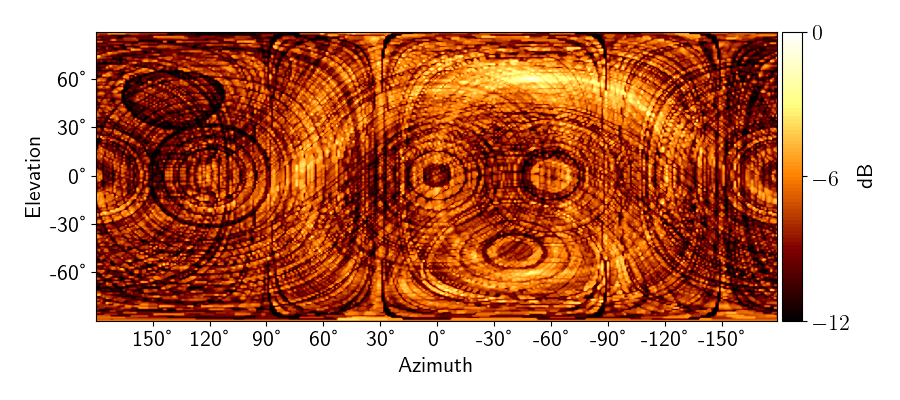
\includegraphics[width=0.8\textwidth]{Figures//Ind4mic1srcProdNeg10Corr.png}
\end{subfigure}
\caption{Figures depict from top-to-bottom level corrected product-SRP-PHAT localization results with SNR = 20dB, SNR = 0dB, SNR = -10dB}
\label{fig:4mic2srcNoisyCompare}
\end{figure}
\subsubsection{Minimum power SRP-PHAT}
Another deconvolution approach can be to use the far-field assumption again, to assume that the power received from a single source to all microphone pairs is the same. In that case, if, the minimum power between the microphone pair is assumed to be the true power (instead of summing), peaks which are detected only by a subset of microphone arrays would disappear automatically and the deconvolution problem can be solved directly. Fig. \ref{fig:4mic1srcNoisyMinPow} shows the results. Even in adverse conditions of 0 dB, the algorithm is fairly able to detect the source at $(50\degree, 60\degree)$, without any subsidiary peaks due to the localization cones. 
\begin{figure}[H]
    \centering
    \begin{subfigure}[b]{0.96\textwidth}
    \centering
    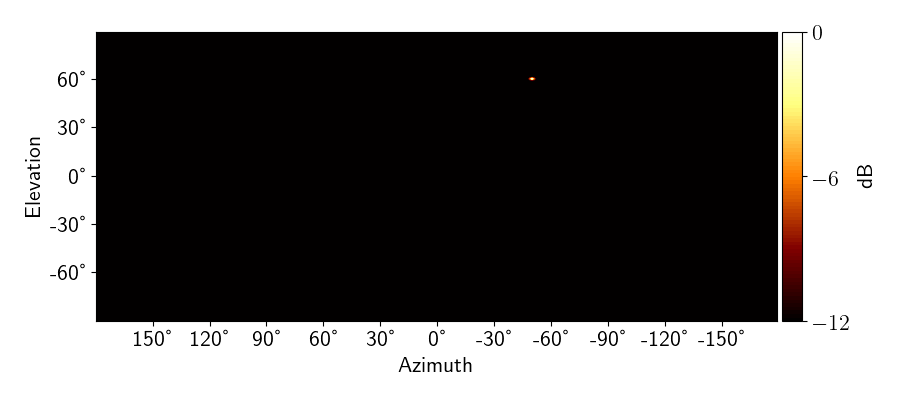
\includegraphics[width=0.8\textwidth]{Figures/Ind4mic1srcMin20.png}
\end{subfigure}
\vskip \baselineskip
\begin{subfigure}[b]{0.96\textwidth}
    \centering
    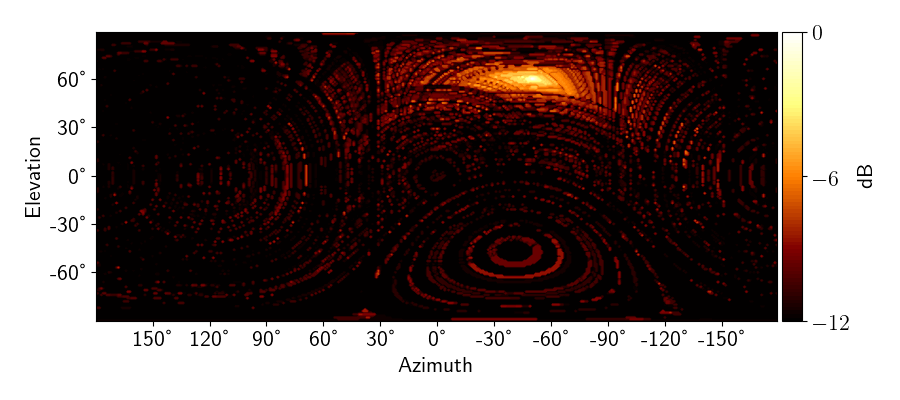
\includegraphics[width=0.8\textwidth]{Figures/Ind4mic1srcMin0.png}
\end{subfigure}
\vskip \baselineskip
\begin{subfigure}[b]{0.96\textwidth}
    \centering
    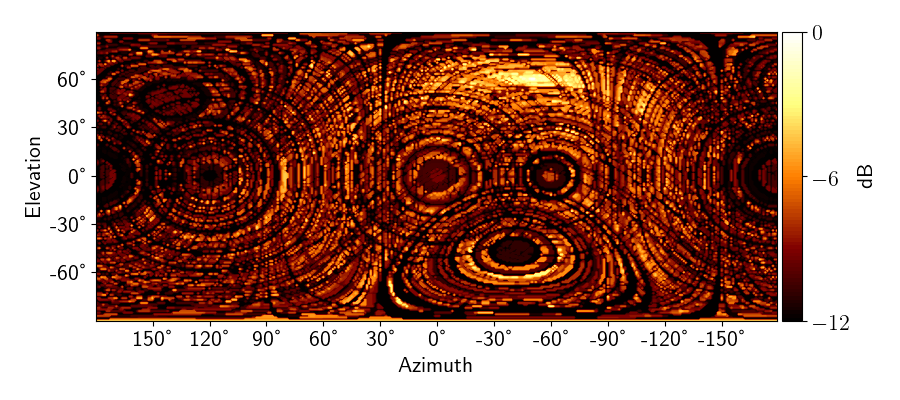
\includegraphics[width=0.8\textwidth]{Figures/Ind4mic1srcMinNeg10.png}
\end{subfigure}
\caption{Figures depict from top-to-bottom minimum power SRP-PHAT localization results with SNR = 20dB, SNR = 0dB, SNR = -10dB}
\label{fig:4mic1srcNoisyMinPow}
\end{figure}
Minimum power SRP-PHAT is same in principle to finding the intersection of multiple cones, since this method only returns sound sources detected by all independent microphone pair cones. The drawback of both product-SRP-PHAT and Minimum power SRP-PHAT is that in case of localizing point sources, even a minor error in temperature or wind recordings has the potential of not detecting the sound source completely. However, since outdoor sound sources are usually large, the cones from microphone pairs are not sharp circular lines, rather, they are broad depending on the sound source size. An error in weather conditions would then cause these fatty circles to `smudge' together. Since minimum power picks the lowest powered circle for each point searched, this has the potential to underestimate the sound source, both in size and magnitude. The advantages of Minimum power SRP-PHAT however are manifold. It removes all subsidiary pseudo peaks while preserving the relative SPL difference between the sources. For example, if 2 sources are located on the same localization cone for a pair of microphones and normal SRP-PHAT is conducted, both sources would appear higher in magnitude than they actually are. Fig. \ref{fig:2srcsSameCone} describes this affect. 
\begin{figure}[H]
    \centering
    \begin{subfigure}[b]{0.96\textwidth}
    \centering
    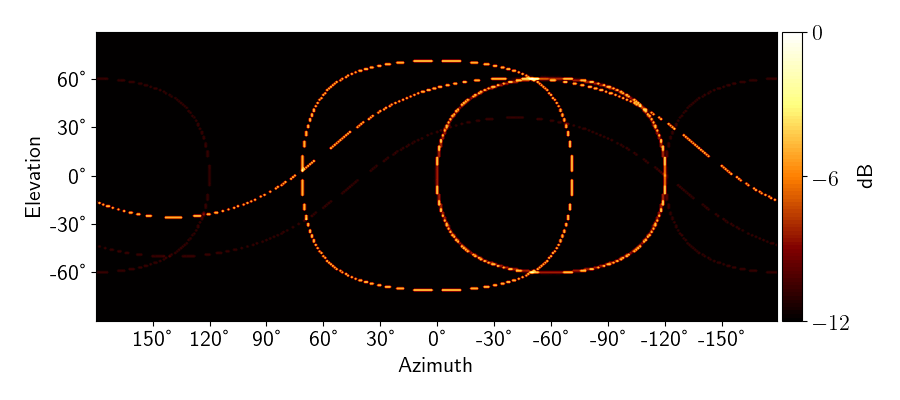
\includegraphics[width=0.8\textwidth]{Figures/2SrcNorm.png}
\end{subfigure}
\vskip \baselineskip
\begin{subfigure}[b]{0.96\textwidth}
    \centering
    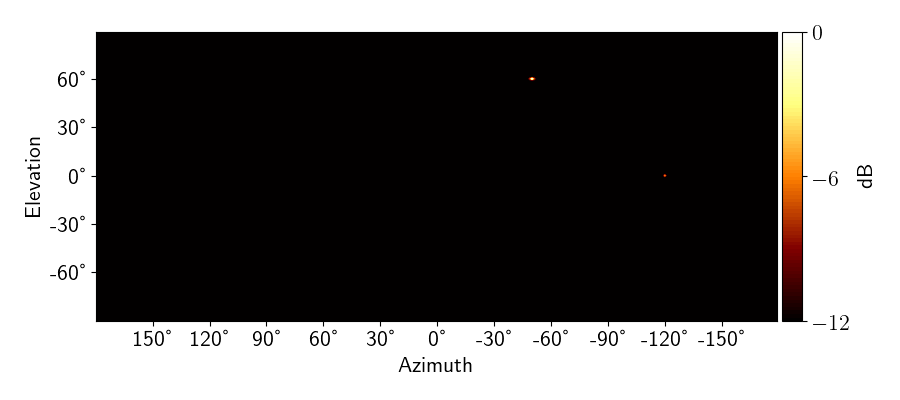
\includegraphics[width=0.8\textwidth]{Figures/2SrcMin.png}
\end{subfigure}
\caption{Figures depict localization results for sources at $(50\degree,60\degree)$ having magnitude 0 dB and $(120\degree,0\degree)$ having magnitude -6 dB, for normal SRP-PHAT (top) and minimum power SRP-PHAT (bottom). In normal SRP-PHAT power from the source at $(50\degree,60\degree)$ is affecting the result for the source at $(120\degree,0\degree)$ since they share a localization circle. }
\label{fig:2srcsSameCone}
\end{figure}
Image sources due to reflection will also have the correct power due to the same reason. So, minimum power SRP-PHAT automatically takes care of the errors due to reflection discussed before in Fig. \ref{fig:4mic1srcRef}. \\
With minimum power SRP-PHAT, the redundant pair information would always improve results in low SNR conditions. This is because only the lowest power from all possible microphone pairs be used. The redundant pair information will thus result in removal or lowering of results in the non-source position due to noise. Fig. \ref{fig:minSRPDep} describes this affect. 
\begin{figure}[H]
    \centering
    \begin{subfigure}[b]{0.96\textwidth}
    \centering
    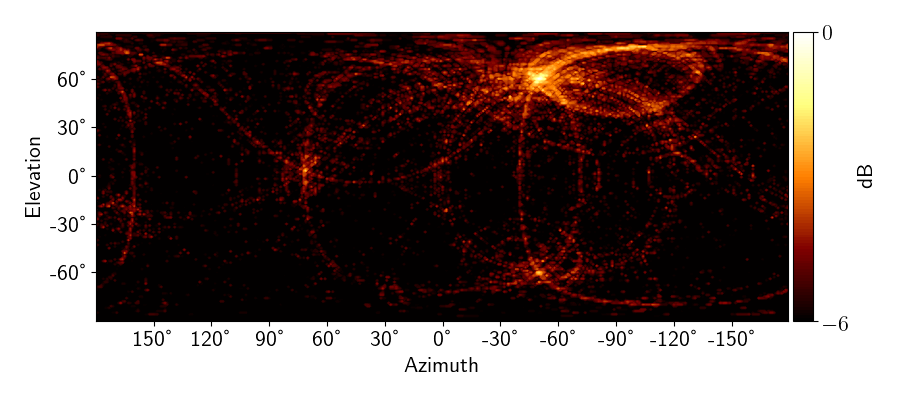
\includegraphics[width=0.8\textwidth]{Figures/Dep4mic1srcResNeg10LowDyn.png}
\end{subfigure}
\vskip \baselineskip
\begin{subfigure}[b]{0.96\textwidth}
    \centering
    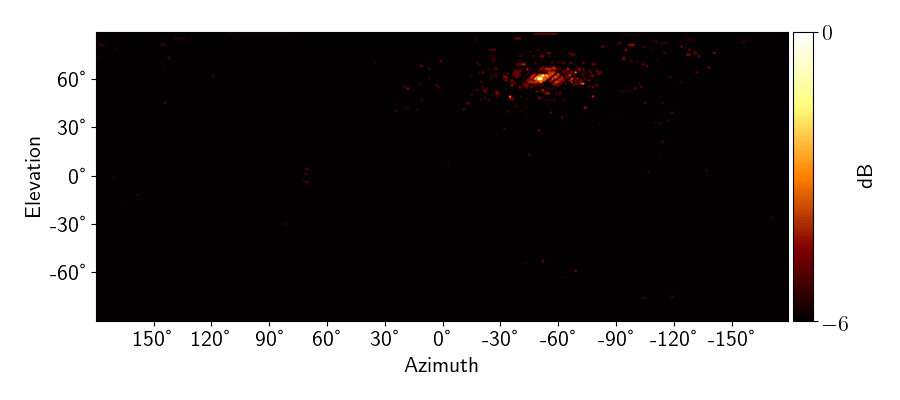
\includegraphics[width=0.8\textwidth]{Figures/Dep4mic1srcResNeg10LowDynMinPow.png}
\end{subfigure}
\caption{Figures depict localization results for source at $(50\degree,60\degree)$ for minimum power SRP-PHAT with only independent microphone pairs (top) and minimum power SRP-PHAT with all microphone pairs (bottom). As expected, using all microphone pairs results in removal of some of the incorrect results from the independent microphone pairs.}
\label{fig:minSRPDep}
\end{figure}


